\section{Langkah-Langkah Percobaan}
\subsection{Persiapan Alat dan Bahan}
Sebelum memulai praktikum ini, praktikan mempersiapkan beberapa alat dan bahan yang diperlukan. Alat dan bahan yang praktikan bawa sendiri diantaranya, laptop yang sudah terinstall Winbox, dan kabel UTP. Sedangkan alat dan bahan yang telah disediakan adalah 1 set router mikrotik. Pengambilan dilakukan oleh perwakilan kelompok.

\subsection{NAT \& Firewall}
\begin{enumerate}
  \item Pemasangan kabel \\
  Praktikan memasang kabel pada router dan laptop sesuai topologi yang diberikan asisten praktikum. Kabel internet disambungkan ke ether 1. Sedangkan laptop disambungkan ke ether 7.
  \item Reset dan Login Router \\
  Sebelum memulai praktikum, router direset terlebih dahulu untuk menghilangkan semua konfigurasi awal. Kemudian, praktikan login kembali ke router.
  \item Konfigurasi DHCP Client \\
  Agar dapat terhubung dengan internet, praktikan mengkonfigurasi ether 1 sebagai DHCP client yang dapat menerima IP dari internet. Konfigurasi ini dilakukan dengan masuk ke menu IP > DHCP Client kemudian menambahkan input baru dengan konfigurasi sesuai modul. Untuk mengecek apakah konfigurasi sudah berhasil, praktikan cek status bound pada DHCP CLient dan ping 8.8.8.8 melalui terminal router.
  \item Konfigurasi IP \\
  Praktikan mengatur IP untuk ether 7 sesuai dengan konfigurasi modul, yaitu 192.168.10.1/24. Hal ini dilakukan pada menu IP > Addresses.
  \item Konfigurasi DHCP Server \\
  Pada praktikum ini, router juga berperan sebagai DHCP server untuk koneksi melalui ether 7. Praktikan mengkonfigurasinya pada menu IP > DHCP Server dengan isi sesuai arahan modul. Alamat yang digunakan disesuaikan dengan alamat network ether 7 yaitu 192.168.10.0/24.
  \item Konfigurasi NAT \\
  Selanjutnya, praktikan mengkonfigurasi NAT. Konfigurasi dilakukan di menu IP > Firewall > NAT dengan pengaturan sesuai modul. Untuk menguji apakah NAT sudah terkonfigurasi dengan baik, praktikan melakukan ping 8.8.8.8 melalui terminal laptop.
  \item Konfigurasi Firewall untuk Semua Situs\\
  Firewall yang dipasang praktikan akan memblokir seluruh akses ke situs manapun. Prkatikan melakukan konfigurasi pada menu IP> Firewall > FIlter Rule dengan isi sesuai modul. Praktikan menguji hasil konfigurasi ini dengan akses pada browser dan hasilnya semua situs tidak dapat dijangkau.
  \item Konfigurasi Firewall untuk Situs Tertentu\\
  Kemudian, praktikan juga mencoba memblokir akses pada situs khusus dengan keyword "speedtest". Hasilnya, situs speedtest tidak dapat dijangkau namun praktikan tetap bisa mengakses situs lain. 
  \item Konfigurasi Bridge pada Router B \\
  Praktikan akan membuat router B menjadi bekerja selayaknya hub/switch. Untuk melakukannya, praktikan menambahkan bridge yang diatur melalui menu Bridge. Selanjutnya, agar router A dapat langsung terhubung dengan interface lain di router B, praktikan menambahkan port (interface) yang akan dijadikan 1 bridge dengan ether 6 (router A), yaitu ether 7. Untuk mengecek apakah konfigurasi sudah berhasil, praktikan mengecek ipconfig pada laptop 2 yang terhubung dengan router B di ether 7. Ternyata tidak berhasil. 
  \item Konfigurasi DHCP Server lagi \\
  ntuk melayani kebutuhan IP di router B, praktikan membuat DHCP server untuk interface ether 6 yang terhubung ke router B. Untuk mengetahui hasilnya, praktikan mengecek ipconfig dan laptop 2 ternyata sudah mendapatkan IP. Praktikan kemudian mengecek koneksi intenet dari laptop 2. Ditemukan laptop 2 dapat mengakses internet.
\end{enumerate}

\section{Analisis Hasil Percobaan}
Pada praktikum ini, praktikan menemui beberapa kendala yang sebenarnya menjurus ke penggunaan dan fungsi sebenarnya NAT (network Address Translation) dan Firewall. Penggunaan NAT di praktikum ini fokus pada keperluan untuk akses jaringan luar dari jaringan lokal. Keperluan ini diwujudkan dengan adanya NAT, dimana router dengan akses internet, perlu melakukan translasi ip jaringan lokal untuk selanjutnya meneruskan komunikasi ke internet. Ketika jaringan lokal tidak memiliki NAT, ia tetap dapat berkomunikasi dengan device lain di lokal, namun tidak ke internet. Hal ini selaras dengan teori fungsi NAT yang memungkinkan 1 IP publik router bisa digunakan bersama-sama oleh beberapa perangkat di lokal. Berkaitan dengan NAT pula, konfigurasinya ternyata bisa di defaultkan agar dapat melakukan translasi dari seluruh subnet yang ada di network. Pada percobaan firewall, praktikan semakin memahami bagaima fungsi firewall untuk blocking akses.  Percobaa firewall pertama, praktikan berhasil memblokir semua koneksi yang berasal dari ether 1 atau di dasar teori disebut sebagai packet filtering. Pada mekanisme ini, koneksi diblokir berdasarkan sumber asalnya. Praktikan juga mencoba memblokir koneksi berdasarkan content. Firewall ini disebut juga sebagai application level firewall karena ia mendeteksi kata kunci pada url, jenis konten, dan lain sebagainya.

\section{Hasil Tugas Modul}
Sampai waktu saya mengerjakan (8 Juni 2025 pukul 10.40 WIB), tugas modul belum tersedia. 
\begin{figure}[h]
    \centering
    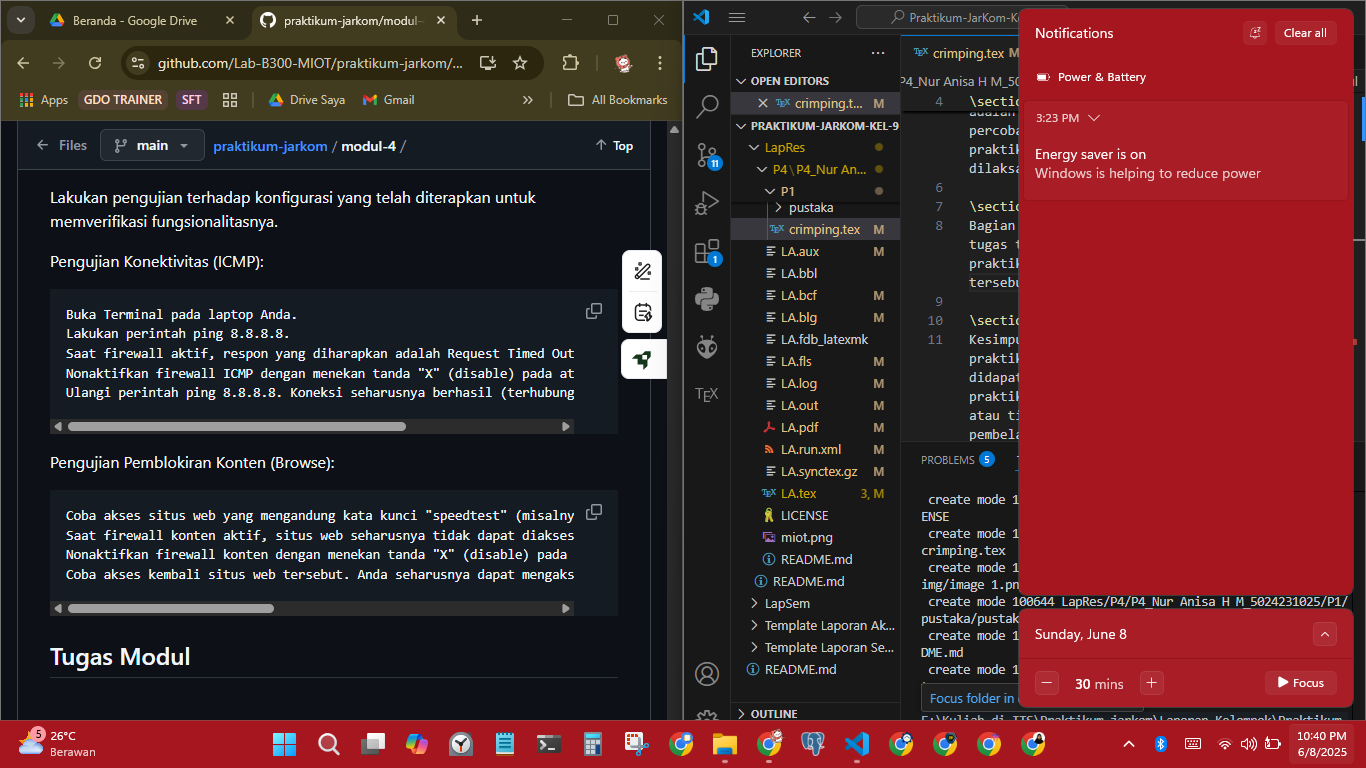
\includegraphics[width=0.5\textwidth]{tumod/notumod.png}
    \caption{Tugas Modul}
    \label{fig:tugas-modul}
\end{figure}

\section{Kesimpulan}
Berdasarkan praktikum yang telah dilakukan, dapat diambil beberapa kesimpulan penting. Pertama, agar koneksi lokal dapat berkomunikasi dengan internet melalui 1 IP address publik diperlukan NAT. Kedua, NAT dapat berlaku 1 untuk semua meskipun network lokal terbagi-bagi. Ketiga, firewall dapat meblokir akses komunikasi, baik berdasarkan isi content nya maupun port inputnya.

\section{Lampiran}
\begin{figure}[h]
    \centering
    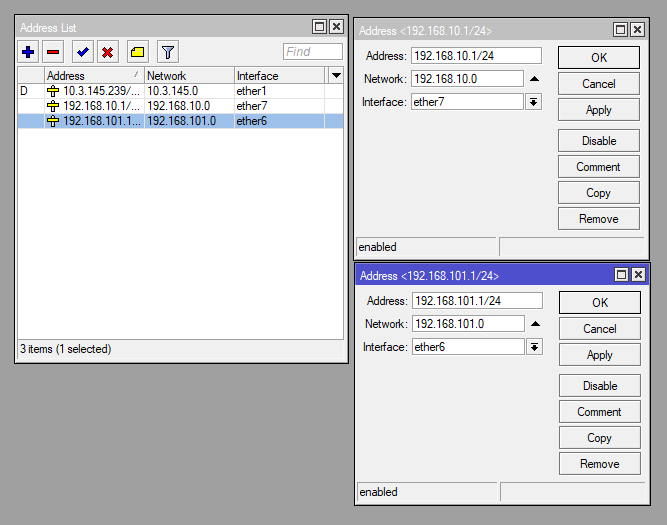
\includegraphics[width=0.5\textwidth]{dokum/Addreses R1.png}
    \caption{Menambahkan IP Address pada Router 1}
    \label{fig:addressr1}
\end{figure}
\begin{figure}[h]
    \centering
    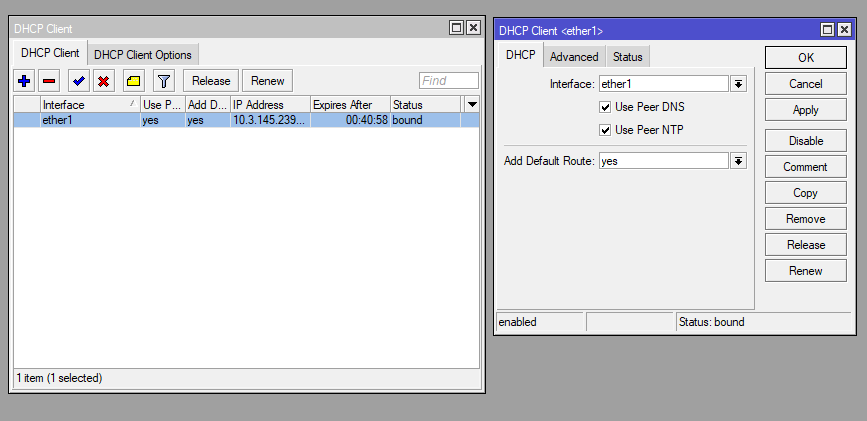
\includegraphics[width=0.5\textwidth]{dokum/dhcp client r1.png}
    \caption{Menkonfigurasi Router A sebagai DHCP Client}
    \label{fig:DHCPclientr1}
\end{figure}
\begin{figure}[h]
    \centering
    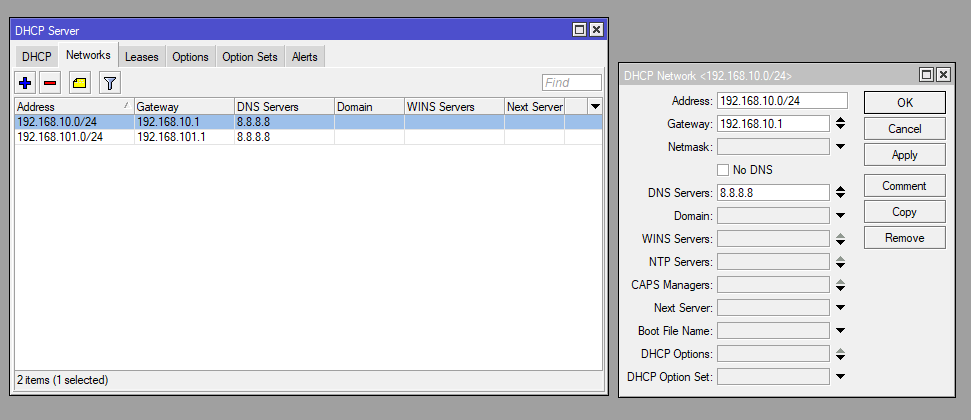
\includegraphics[width=0.5\textwidth]{dokum/dhcp server r1.png}
    \caption{Menkonfigurasi Router A sebagai DHCP Server}
    \label{fig:DHCPserverr1}
\end{figure}
\begin{figure}[h]
    \centering
    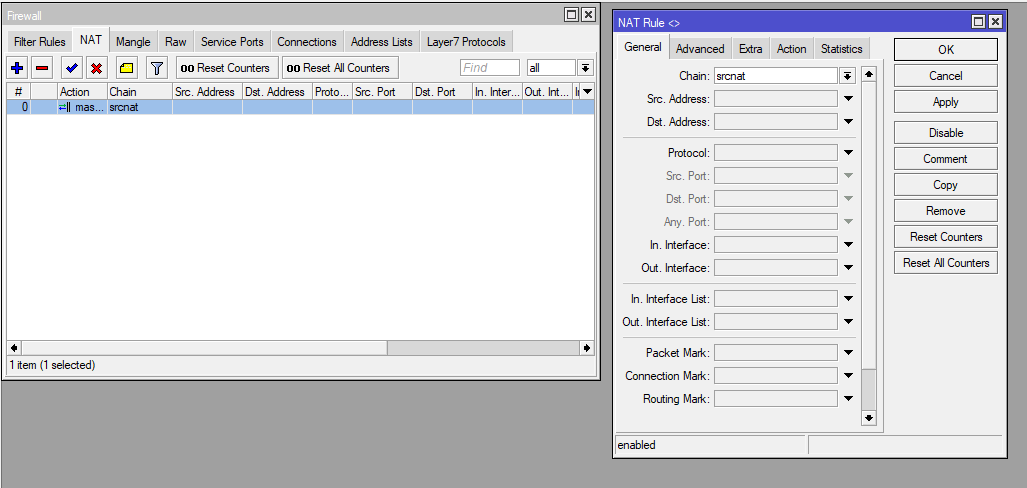
\includegraphics[width=0.5\textwidth]{dokum/NAT r1.png}
    \caption{Konfigurasi NAT pada Router A}
    \label{fig:nat-ra}
\end{figure}
\begin{figure}[h]
    \centering
    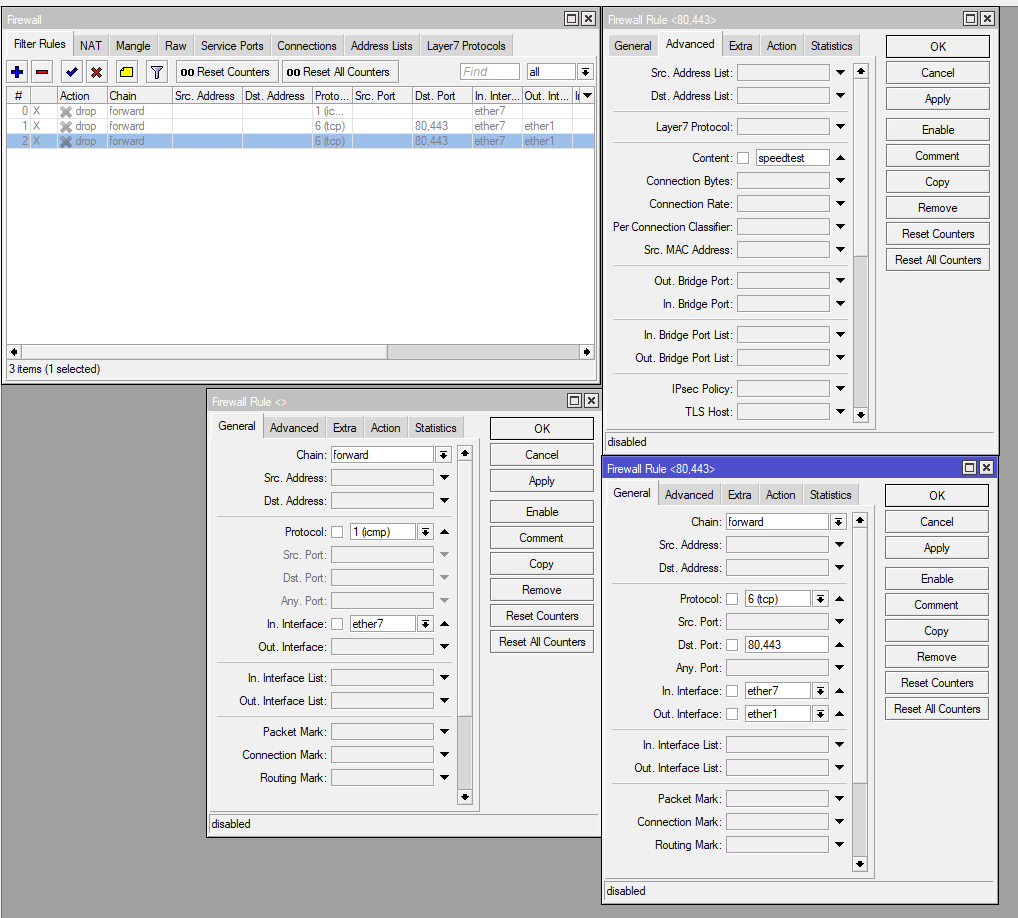
\includegraphics[width=0.5\textwidth]{dokum/filter rule r1.png}
    \caption{Konfigurasi Firewall pada Router A}
    \label{fig:firewall-ra}
\end{figure}

\subsection{Dokumentasi saat praktikum}
\begin{figure}[h]
    \centering
    % \includegraphics[width=0.5\textwidth]{nama_file_gambar.jpg}
    \caption{Dokumentasi Praktikum}
    \label{fig:dokum}
\end{figure}